\chapter{Materials \& Methods}

\section{Chapter Overview}
This chapter describes the materials, datasets, software, and methods used to design, build, and evaluate the clinical Retrieval-Augmented Generation (RAG) system. It documents data sources and governance, preprocessing and chunking procedures, embedding and indexing choices, the retrieval and LLM orchestration pipeline, interfaces for access (API, frontend, CLI), and the evaluation protocol.

\subsection{Process overview}
The main challenge in this work is connecting static hospital records with a system that can have conversations about patient care. Traditional medical information systems use keyword searches or database queries, which cannot capture the complex, context-dependent nature of medical thinking. This project creates a new way to interact with clinical data by building a pipeline that turns raw hospital records into a smart conversational system that can answer medical questions with evidence-based responses.


The approach covers the full process from getting data to deploying the system: we start with structured hospital records and convert them step-by-step into searchable knowledge that understands meaning. This knowledge is then managed by a smart search system that understands medical context, limits searches to the right patient admissions or medical areas, and puts together focused evidence. Finally, a language model running locally combines this evidence into clear, well-cited responses while staying strictly grounded in facts to prevent medical errors.

This complete approach allows natural language conversations with complex medical data while keeping the accuracy, transparency, and safety needed for healthcare uses. The detailed sections that follow explain each part of this pipeline, from the first data processing choices to the final testing methods used to check how well the system works.

% Removed FloatBarrier to avoid forcing a layout break before the figure



% ========================
% 3.1 System Overview
% ========================
\section{System Overview}

This design follows a clear separation of responsibilities: a data creation and processing layer that normalises and chunks raw EHR tables into searchable documents; an embedding and vector store layer that encodes and indexes those chunks for semantic retrieval; a lightweight coordination layer that constrains retrieval by admission/section and prepares compact evidence contexts; and a model/serving layer that hosts small, locally runnable LLMs and exposes user-facing APIs and a web UI. This structure prioritises traceability, privacy, and reproducibility while keeping runtime costs and latency manageable for local experiments.
\begin{figure}[H]
  \centering
  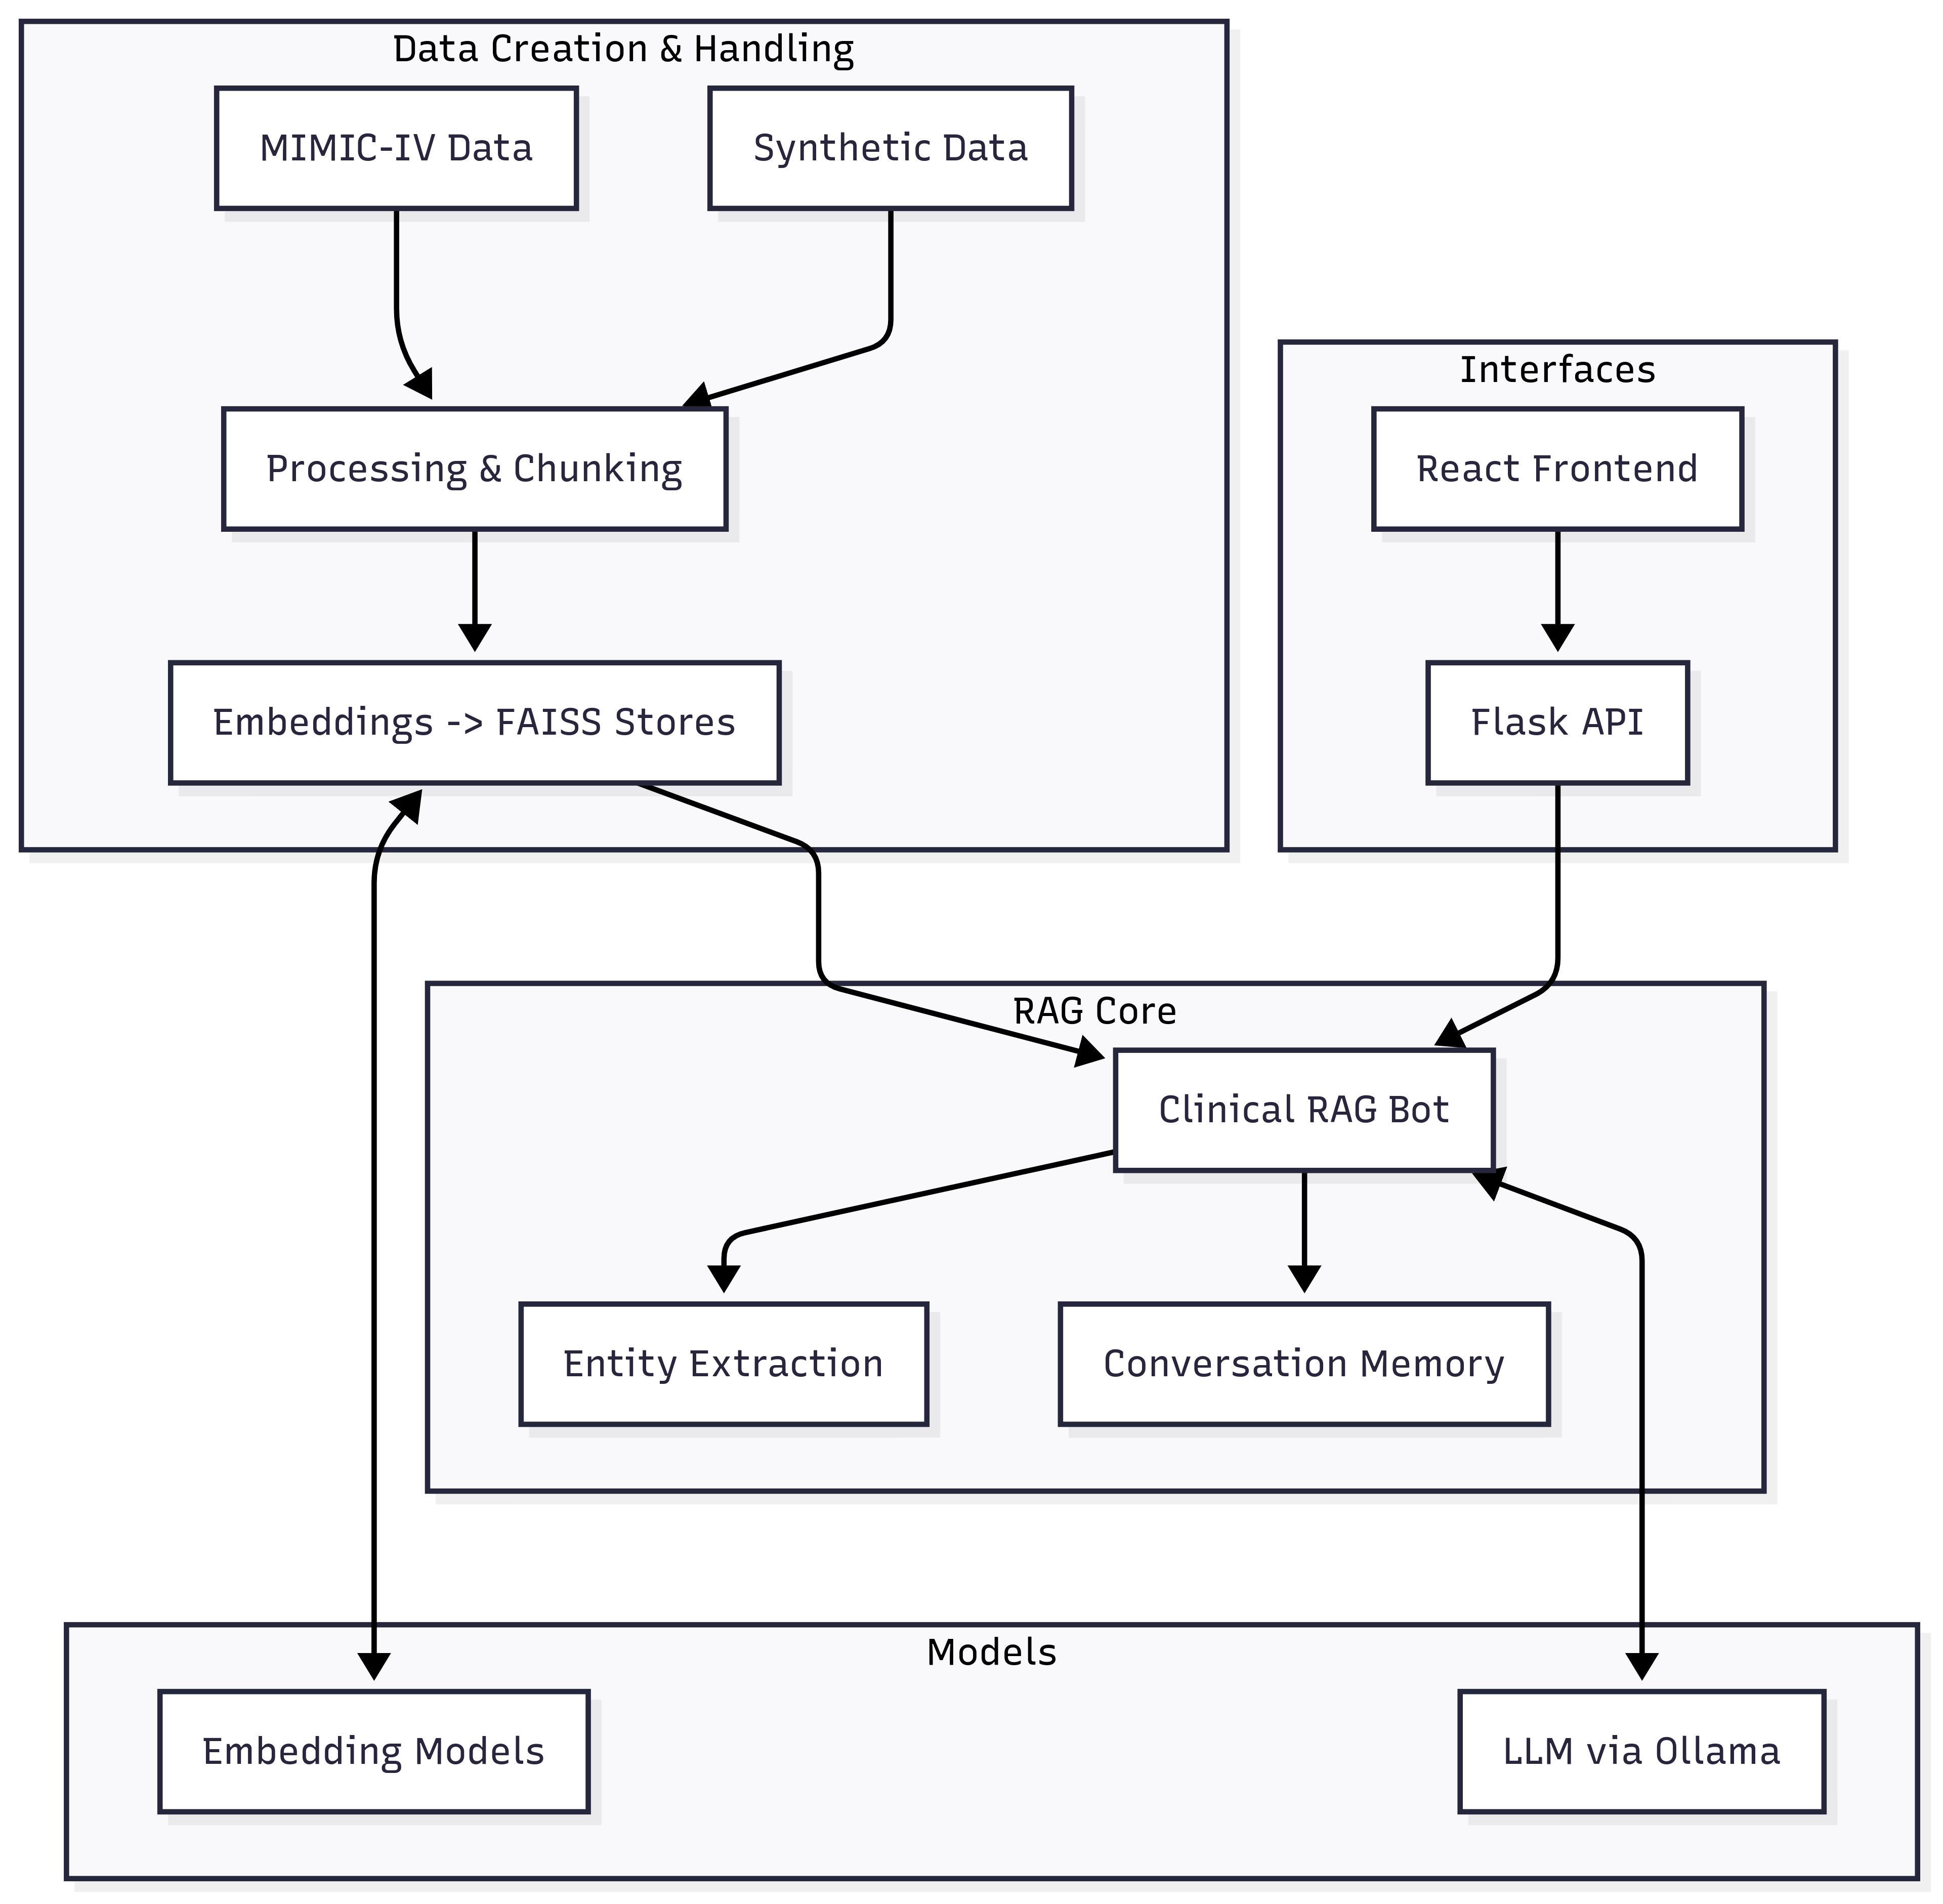
\includegraphics[width=0.95\linewidth]{chap3_methodology/images/system_archi.png}
<<<<<<< HEAD
  \caption{System architecture. Image file: \texttt{chap3_methodology/images/system_archi.png} (label: \texttt{fig:system_architecture})}
=======
  \caption{System architecture}
>>>>>>> 3fc1d716e5d0a4e382e6763c197397e68de6ba0e
  \label{fig:system_architecture}
\end{figure}


% ========================
% 3.2 Data Sources and Governance
% ========================
\section{Data Sources and Governance}

\subsection{Datasets}
\begin{itemize}
  \item Real data: MIMIC-IV sample exports are stored under \texttt{mimic\_sample\_1000/}.
  \item Synthetic data: A generator in \texttt{synthetic\_data/} produces structurally consistent, fictional clinical records for development/demo when real data are unavailable.
\end{itemize}

\noindent A data provider abstraction (\texttt{RAG\_chat\_pipeline/utils/data\_provider.py}) automatically chooses real vs. synthetic sources, preferring real MIMIC-derived exports when present.

\subsection{Ethics and Access}
Use of MIMIC-IV requires credentialed access and adherence to PhysioNet data use agreements. Public artefacts in this project are restricted to code and synthetic data. The system is intended for research/education purposes only and should not be used for clinical decision-making.

% ========================
% 3.3 Software, OS, and Runtime Environment
% ========================
\section{Software, OS, and Runtime Environment}
Experiments were executed on Microsoft Windows (user environment), Python 3.11, and React.js for the frontend.

\smallskip
\noindent\textbf{Representative versions:}
\begin{itemize}
  \item Python: 3.11
  \item Node.js: \(\ge\) 16 (v18+ recommended)
  \item LangChain: 0.3.25; \texttt{langchain-community}: 0.3.24
  \item FAISS CPU: 1.11.0; sentence-transformers: 4.1.0
  \item Torch: 2.7.1; Transformers: 4.52.4
  \item Flask: 3.0.2; Flask-CORS: 4.0.1
  \item Ollama: 0.5.1 (models pulled locally)
\end{itemize}

% ========================
% 3.4 System Configuration
% ========================
\section{System Configuration}
Central configuration is defined in "\texttt{RAG\_chat\_pipeline/config/config.py}".

\noindent Embedding model nicknames map to HuggingFace model IDs and vector-store directories. The LLM model set is managed via Ollama. Unless otherwise specified, the session-level defaults set by \texttt{set\_models()} select \texttt{S-PubMedBert-MS-MARCO} embeddings and \texttt{deepseek-r1:1.5b} as the LLM. Alternative combinations are supported for evaluation: \texttt{all-MiniLM-L6-v2}, \texttt{multi-qa-mpnet-base-cos-v1}, \texttt{BiomedNLP-PubMedBERT}, \texttt{e5-base-v2}, \texttt{BioLORD-2023-C}, \texttt{BioBERT}, \texttt{S-PubMedBert-MedQuAD}; and LLMs such as Qwen3, Llama 3.2, Gemma 2B, Phi-3, TinyLlama).

% ========================
% 3.5 Data Processing and Document Construction
% ========================
\section{Data Processing and Document Construction}

\subsection{Preprocessing}
We prepared data with notebooks in \texttt{data\_handling/}. Sampling was performed at the admission level to produce a working subset (\texttt{mimic\_sample\_1000/}) by selecting a fixed-size random sample of \texttt{hadm\_id}s and joining the primary tables (diagnoses, procedures, labs, microbiology, prescriptions) on \texttt{hadm\_id} and \texttt{subject\_id}. This preserves cross-table coherence while controlling index size and memory footprint.

\noindent Key preprocessing steps:
\begin{enumerate}
  \item Normalise column names and types (e.g., enforce integer \texttt{hadm\_id}, \texttt{subject\_id})
  \item Map each row to a semantically labeled section: \texttt{header}, \texttt{diagnoses}, \texttt{procedures}, \texttt{labs}, \texttt{microbiology}, \texttt{prescriptions}
  \item Compose section-scoped textual records embedding key fields (codes, values/units, dates) and attach metadata
\end{enumerate}

\subsection{Chunking}
Documents are segmented into meaningful chunks optimised for clinical QA. We apply section-aware chunking before size-based splitting so that each chunk stays on the same topic (e.g., lab results grouped, diagnoses grouped). Chunk sizes of 600--900 characters with 80--150 character overlap worked well in practice for our lightweight local LLMs (balancing recall and context-window constraints). Metadata (\texttt{hadm\_id}, \texttt{subject\_id}, \texttt{section}) is preserved on every chunk to enable admission- and section-scoped retrieval.

\smallskip
\noindent An illustrative chunking routine:
\begin{minted}[fontsize=\footnotesize, breaklines]{python}
from langchain_text_splitters import RecursiveCharacterTextSplitter

SECTION_SEPARATORS = ["\n\n", "\n", ". ", " "]

def chunk_clinical_text(text: str, chunk_size=800, chunk_overlap=120):
    splitter = RecursiveCharacterTextSplitter(
        chunk_size=chunk_size,
        chunk_overlap=chunk_overlap,
        separators=SECTION_SEPARATORS,
        is_separator_regex=False,
    )
    return splitter.split_text(text)
\end{minted}

\noindent The notebooks emit a list of \texttt{langchain.schema.Document} with \texttt{page\_content} and \texttt{metadata}, saved to \texttt{mimic\_sample\_1000/chunked\_docs.pkl} (or synthetic equivalent). These chunks are the source for vector indexing.

% ========================
% 3.6 Embeddings and Vector Stores
% ========================
\section{Embeddings and Vector Stores}

\subsection{Model Setup}
The embedding manager (\texttt{RAG\_chat\_pipeline/core/embeddings\_manager.py}) loads a SentenceTransformers model by nickname from config, caching it under \texttt{models/<model-name>/}. If not present locally, it is downloaded and saved. A \texttt{HuggingFaceEmbeddings} wrapper provides the LangChain interface.

\subsection{FAISS Indexing}
For each embedding configuration, a FAISS vector store is created from the chunked documents and saved under \texttt{vector\_stores/<store-name>/}. On startup, the system attempts to load the existing store; if missing, it builds a new one and persists both the index and the chunked corpus.

% ========================
% 3.7 RAG Pipeline and Inference
% ========================
\section{RAG Pipeline and Inference}

\subsection{RAG Contract (inputs, outputs, guardrails)}
  	extbf{Inputs:} user query; optional \texttt{hadm\_id}, \texttt{subject\_id}, \texttt{section}; optional \texttt{chat\_history} (last N messages).\\
  	extbf{Outputs:} answer text with inline citations; list of cited document IDs/sections; small diagnostics (retrieval mode, \(k\) used).\\
  	extbf{Invariants:} ground answers strictly in retrieved content; if evidence is missing, state ``Not found in records''; always append a standard disclaimer.\\
  	extbf{Constraints:} \(k \le 5\); per-section line caps in the structured context; bounded context window and per-call timeout.

\subsection{Retrieval steps (high level)}
1) Parse identifiers/section from the query and recent history (regex).\\
2) Build a candidate set using in-memory indices if hints exist; otherwise, consider the full corpus.\\
3) Rank candidates with FAISS vector similarity.\\
4) Keep top-\(k\) (default \(k=5\)).\\
5) Compact into a single structured, section-aware context (limit lines per section; prefer ICD patterns, dosages, and numeric labs).\\
6) Generate with a prompt that enforces grounding and citations.

\noindent Minimal pseudocode (illustrative):
\begin{minted}[fontsize=\footnotesize, breaklines]{python}
ids = parse_hints(query, chat_history)  # hadm_id, subject_id, section
candidates = build_candidates(ids)  # from in-memory indices or full corpus
ranked = faiss_rank(candidates, query)
topk = ranked[: min(k, 5)]
context = make_structured_context(topk)  # section-aware, line-capped
answer = llm_answer(query, context, prompt=CLINICAL_PROMPT)
return answer
\end{minted}

\subsection{Retriever}
Given a query, the pipeline first attempts metadata-constrained retrieval when a \texttt{hadm\_id}, \texttt{subject\_id}, or \texttt{section} is available. Efficient in-memory indices (built at bot initialisation) map identifiers and sections to candidate document IDs, reducing the search space before semantic ranking. Otherwise, a global FAISS similarity search is performed.

\smallskip
\noindent At initialisation, the bot builds light-weight Python indices for fast filtering:
\begin{minted}[fontsize=\footnotesize, breaklines]{python}
from collections import defaultdict

self.hadm_id_index = defaultdict(list)
self.subject_id_index = defaultdict(list)
self.section_index = defaultdict(list)
self.hadm_section_index = defaultdict(list)

for i, doc in enumerate(self.chunked_docs):
    hadm = doc.metadata.get("hadm_id")
    sec = str(doc.metadata.get("section", "")).lower()
    if hadm is not None:
        try:
            hadm_i = int(hadm)
            self.hadm_id_index[hadm_i].append(i)
            if sec:
                self.hadm_section_index[(hadm_i, sec)].append(i)
        except ValueError:
            pass
    if sec:
        self.section_index[sec].append(i)
\end{minted}

\noindent When a \texttt{hadm\_id} or \texttt{section} is present, only the corresponding candidate set is ranked semantically.

\subsection{Context Construction}
Top-$k$ (default \(k=5\), bounded for performance) documents are semantically ranked. For efficiency and to improve answer formatting, the system extracts concise, section-aware snippets (diagnoses, procedures, labs, prescriptions, microbiology, header) and composes a single structured context document passed to the LLM. Rules favour lines with section-specific keywords and patterns (e.g., ICD codes, dosages, numeric lab values/units) while limiting per-section lines to keep within context windows.

\subsection{LLM Answering}
Answers are generated using an Ollama-hosted model (default DeepSeek-R1 1.5B) through LangChain's \texttt{create\_stuff\_documents\_chain}, with a prompt that enforces the guardrails below.

\noindent \textbf{Prompt guardrails:}
\begin{itemize}
  \item Cite sources inline and include codes/values/units/dates when present
  \item If evidence is missing, say so; do not guess
  \item Respect admission/section scope when provided
  \item Always append the standard disclaimer
\end{itemize}

\subsection{Entity Extraction and Conversational Context}
A deterministic regex-based extractor (\texttt{helper/entity\_extraction.py}) identifies \texttt{hadm\_id}, \texttt{subject\_id}, and \texttt{section} hints from the current query and recent chat messages. For follow-ups, an LLM-powered rephrasing step condenses the question into a standalone form while preserving identifiers. Chat history is truncated to a configurable maximum (\textbf{60 messages}; see \texttt{MAX\_CHAT\_HISTORY} in config) to control context length.

\subsection{RAG Core Emphasis and Design Evolution}
The initial blueprint used a straightforward vector index + chat engine with strict context mode:
\begin{minted}[fontsize=\footnotesize, breaklines]{python}
from llama_index.core import VectorStoreIndex, SimpleDirectoryReader
from llama_index.embeddings.ollama import OllamaEmbedding
from llama_index.llms.ollama import Ollama

docs = SimpleDirectoryReader("./parsed_emails").load_data()
embed_model = OllamaEmbedding(model_name="nomic-embed-text")
llm = Ollama(model="llama3.2")

index = VectorStoreIndex.from_documents(docs, embed_model=embed_model)
chat_engine = index.as_chat_engine(
    llm=llm,
    chat_mode="context",
    verbose=True
)
response = chat_engine.chat("There is package mentioned for spaghetti code")
\end{minted}

We attempted a two-step pipeline (LLM judges chunk relevance, then answers), but lightweight local models had small context windows and were unreliable as rankers. The reliable fix was a \textbf{custom retriever}: extract \texttt{hadm\_id}/\texttt{subject\_id}/\texttt{section} via regex/patterns, filter candidates with in-memory indices, reduce content by meaning, then pass only the top snippets to the LLM. The core search is:
\begin{minted}[fontsize=\footnotesize, breaklines]{python}
candidate = self._filter_candidate_documents(hadm_id, subject_id, section, limit=20)
if candidate is None:
    retrieved = self.vectorstore.similarity_search(question, k=min(k, 20))
else:
    retrieved = self._semantic_search_on_docs(candidate, question, k=min(k, 5))
structured = self._extract_clinical_content(retrieved)
prompt = self._create_clinical_prompt(hadm_id, subject_id)
chain = create_stuff_documents_chain(self.llm, prompt)
answer = safe_llm_invoke(chain, {"input": question, "context": [Document(page_content=structured)]})
\end{minted}

% Consolidated hallucination mitigation earlier; avoid repetition here.

% ========================
% 3.8 Interfaces
% ========================
\section{Interfaces}

\subsection{API}
A Flask service in \texttt{api/app.py} exposes endpoints:
\begin{itemize}
  \item \texttt{POST /api/chat}: process a chat message and optional history
  \item \texttt{GET /api/models}: list available embedding models and vector stores
  \item Static serving: production build of the React app
\end{itemize}

\noindent \textbf{Chat endpoint contract (summary):}
\begin{itemize}
  \item Request: \{\texttt{query: str}, optional \texttt{hadm\_id}, \texttt{subject\_id}, \texttt{section}, optional \texttt{history: [\{role, content\}] }\}
  \item Response: \{\texttt{answer: str}, \texttt{citations: [\{doc\_id, section\}]}, \texttt{diagnostics: \{mode, k\}}\}
\end{itemize}

\subsection{Frontend}
A React UI (\texttt{frontend/}) provides a chat interface, model introspection, and sample query suggestions sourced from the data provider.

\subsection{CLI}
\texttt{cli\_chat.py} offers an interactive console with session logging and history management.

% ========================
% 3.9 Challenges and Mitigations
% ========================
\section{Challenges and Mitigations}
  	extbf{Risk: medical hallucinations and sensitive data.} Early versions retrieved globally and over-supplied context, which could produce made-up details. Mitigations:
\begin{itemize}
  \item Admission-/section-scoped retrieval via in-memory indices
  \item Deterministic entity extraction (regex) to avoid LLM-based unexpected settings changes
  \item Structured snippet extraction with section rules
  \item Post-processing to enforce disclaimers and fix citations
\end{itemize}

\noindent Replacing the two-step LLM-as-ranker approach with the custom retriever + semantic re-ranking significantly improved factual grounding on lightweight local models.

\noindent \textbf{Failure modes and fallbacks:}
\begin{itemize}
  \item Missing hints (no IDs/section) \textrightarrow{} use global search
  \item Empty candidate set \textrightarrow{} fall back to global k-NN
  \item FAISS store missing at startup \textrightarrow{} rebuild once, then cache
  \item Timeout or partial retrieval \textrightarrow{} return a safe message without guessing
\end{itemize}

% ========================
% 3.10 Evaluation Protocol
% ========================
\section{Evaluation Protocol}
We provide only a brief overview here; detailed metrics and comparisons are in Results. The evaluator generates category-specific gold questions and computes pass/fail and summary statistics per model combination. We validate against structured signals (ICD patterns, dosages, units) and measure retrieval latency; full scoring details are in Results.

\subsection{Gold Questions and Categories}
Gold questions are created from available records (diagnoses, procedures, labs, etc.) with associated \texttt{hadm\_id}s when applicable. Full evaluation outcomes are reported in Results.

% ========================
% 3.11 Modularity and Extensibility
% ========================
\section{Modularity and Extensibility}
The system is modular: configuration (\texttt{config/}), core RAG components (\texttt{core/}), helpers, utilities, API, and frontend are decoupled. Models are selectable at runtime (\texttt{set\_models()}), and vector stores are tied to embeddings, enabling comparison tests.

% ========================
% 3.12 Reproducibility
% ========================
\section{Reproducibility}

\subsection{Environment Setup}
\begin{enumerate}
  \item Create Python 3.11 env: \texttt{pip install -e .}
  \item Install frontend deps: \texttt{cd frontend \&\& npm install}
  \item Install Ollama and pull models: \texttt{deepseek-r1:1.5b}
\end{enumerate}

\subsection{Data Preparation}
\begin{itemize}
  \item Real data: Place MIMIC-IV exports under \texttt{mimic\_sample\_1000/}, run \texttt{creating\_docs.ipynb}
  \item Synthetic data: Run \texttt{synthetic\_data\_generator.py}
\end{itemize}

\subsection{Running and Evaluation}
\begin{itemize}
  \item API: \texttt{python api/app.py}
  \item UI: \texttt{cd frontend; npm start}
  \item CLI: \texttt{python cli\_chat.py chat}
  \item Quick eval: \texttt{python -m benchmarks.model\_evaluation\_runner single ms-marco deepseek short}
  \item Full comp: \texttt{python -m benchmarks.model\_evaluation\_runner all full}
\end{itemize}

% ========================
% 3.13 Quality Assurance
% ========================
\section{Quality Assurance and Performance}
The chatbot uses in-memory indices for fast filtering and embedding caching. Retrieval sets are capped for latency control. Post-processing normalises outputs.

\noindent \textbf{Deterministic behaviour and caching:} model versions are pinned; random seeds set where applicable; embeddings cached on disk; \(k\) and per-section limits fixed; chat history bounded.

% ========================
% 3.14 Limitations
% ========================
\section{Limitations}
We evaluate on limited MIMIC/synthetic data. Local LLMs (1-4B params) balance privacy/cost but may underperform large models. Results depend on embeddings, chunking, and prompting.

% ========================
% 3.15 Summary
% ========================
\section{Summary}
The methodology provides an end-to-end, reproducible pipeline from MIMIC-compatible data to a clinical RAG system. All components are parameterised to support comparison tests.
